\documentclass{article}

\usepackage{amsmath,amssymb,amsthm}
\usepackage{enumitem}
\usepackage{float}
\def\simp{\text{simp}}

\theoremstyle{definition}
\newtheorem{definition}{Definition}

\theoremstyle{example}
\newtheorem{example}{Example}

\theoremstyle{remark}
\newtheorem*{remark}{Remark}


\setlength{\oddsidemargin}{0.25 in}
\setlength{\evensidemargin}{-0.25 in}
\setlength{\topmargin}{-0.6 in}
\setlength{\textwidth}{6.5 in}
\setlength{\textheight}{8.5 in}
\setlength{\headsep}{0.75 in}
\setlength{\parindent}{0 in}
\setlength{\parskip}{0.1 in}

\newtheorem{theorem}{Theorem}
\newtheorem{corollary}{Corollary}
\newtheorem{proposition}{Proposition}
\newtheorem*{remark}{Remark}
\theoremstyle{definition}
\newtheorem{example}{Example}
\newtheorem{definition}{Definition}

\newcommand{\lecture}[4]{
   \pagestyle{myheadings}
   \thispagestyle{plain}
   \newpage
%   \setcounter{lecnum}{#1}
   \setcounter{page}{1}
   \noindent
   \begin{center}
   \framebox{
      \vbox{\vspace{2mm}
    \hbox to 6.58in { {\bf CSC~565: Graph Theory
                        \hfill North Carolina State University} }
    \hbox to 6.58in { {\bf Fall 2019
                        \hfill Computer Science} }
       \vspace{4mm}
       \hbox to 6.28in { {\Large \hfill Lecture #1: #2  \hfill} }
       \vspace{2mm}
       \hbox to 6.28in { {\it Lecturer: {\it Don Sheehy {\tt <drsheehy@ncsu.edu>}} \hfill Scribe: #4} }
      \vspace{2mm}}
   }
   \end{center}
   \markboth{Lecture #1: #2}{Lecture #1: #2}
   \vspace*{4mm}
}

\usepackage{graphics,tikz}
\begin{document}



  \title{Lecture 3}
  \author{Scribed by: Xianpeng Liu and Yuhan Chen}
  \maketitle




  \begin{definition}
    A \textit{walk} in a graph $G=(V,E)$ is a sequence of vertices $(v_{0},...,v_{k})$ such that $(v_{i-1},v_{i})\in E$ for all $i=1...k$.
  \end{definition}

  \begin{definition}
    A \textit{Euler walk} is a walk that spans every edge exactly once, i.e., $E=\{(v_{i-1},v_{i}) |  i\in \{1...k\}\}$.
  \end{definition}

  \begin{remark}
  A walk is the image of a morphism $P_{k}\to G$. A tour is the image of a morphism $C_{k}\to G$.
  \end{remark}

  \begin{definition}
    Let $G=(V,E)$. Vertices $u,v$ are \textit{connected} if $\exists$ a walk that starts at $u$ and ends at $v$.
  \end{definition}

  \begin{remark}
  We say $G$ is \textit{connected} if $u$ is connected to $v$ for $u,v \in V$.
  \end{remark}


  \begin{theorem}
    Let $G$ be a connected graph. Then, $G$ has an Euler tour iff. the degree of every vertex is even.
  \end{theorem}
  \begin{proof}
    Prove by contradiction. Assume there is no Euler tour. Take longest tour and remove edges. Result still has all even degrees. So, there is a tour that shares $n$ vertex with the longest tour. Combine to get a longer tour and a contradiction.
  \end{proof}

  \begin{definition}
    The \textit{connected components} of a graph are its maximal connected subgraphs.
  \end{definition}
  \begin{remark}
  Connectivity is an Equivalence relation. Equivalence connected components are the subgraphs induced on the equivalence classes of connectivity.
  \end{remark}
  \begin{definition}
    Say $u,v \in V$ are \textit{2-connected} if they remain connected even if I remove any one vertex other than $u,v$.
  \end{definition}
      \begin{figure}[H]
    \centering
      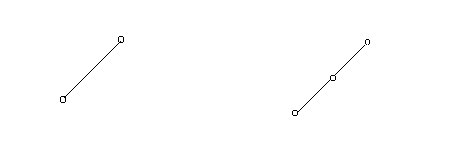
\includegraphics[width=0.48\textwidth]{fig1.png}
      \caption{This graph is not 2-connected}
    \end{figure}
  \begin{definition}
    Say $G$ are \textit{2-connected} if $u,v$ are 2-connected for all $u,v \in V$.
  \end{definition}

  \begin{definition}
    Say $G$ are \textit{k-connected} if $G\setminus S$ is conencted for any subset $S\subset V$ such that $|S|<k$.
  \end{definition}



\end{document}
